% Created by tikzDevice version 0.12.3.1 on 2022-08-16 21:21:16
% !TEX encoding = UTF-8 Unicode
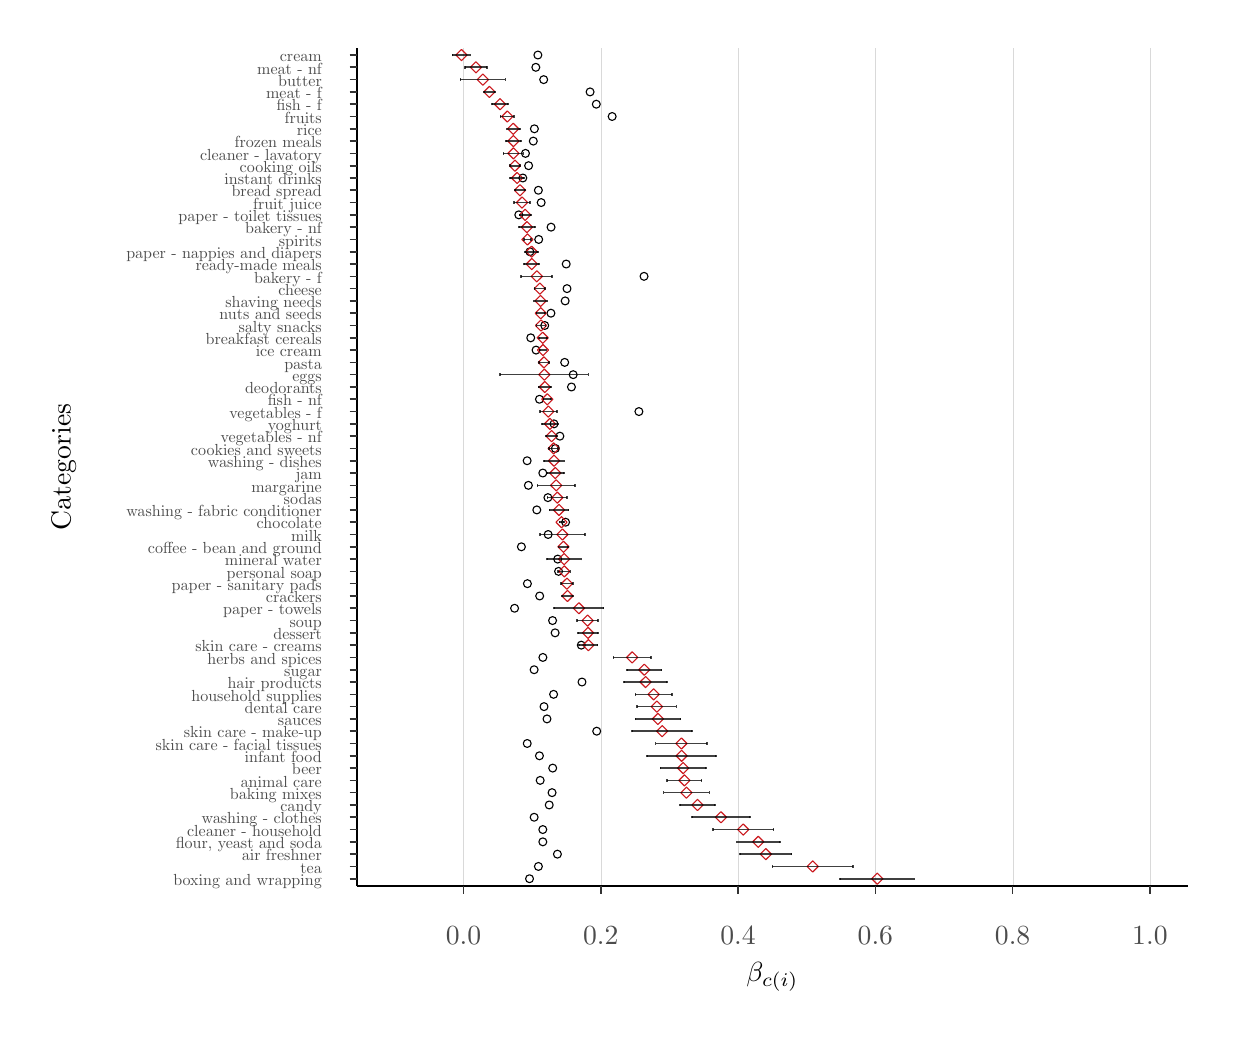
\begin{tikzpicture}[x=1pt,y=1pt]
\definecolor{fillColor}{RGB}{255,255,255}
\path[use as bounding box,fill=fillColor,fill opacity=0.00] (0,0) rectangle (433.62,361.35);
\begin{scope}
\path[clip] (  0.00,  0.00) rectangle (433.62,361.35);
\definecolor{drawColor}{RGB}{255,255,255}
\definecolor{fillColor}{RGB}{255,255,255}

\path[draw=drawColor,line width= 0.6pt,line join=round,line cap=round,fill=fillColor] (  0.00,  0.00) rectangle (433.62,361.35);
\end{scope}
\begin{scope}
\path[clip] (119.04, 51.15) rectangle (419.17,354.12);
\definecolor{drawColor}{RGB}{255,255,255}

\path[draw=drawColor,line width= 0.3pt,line join=round] (132.68, 51.15) --
	(132.68,354.12);

\path[draw=drawColor,line width= 0.3pt,line join=round] (182.29, 51.15) --
	(182.29,354.12);

\path[draw=drawColor,line width= 0.3pt,line join=round] (231.90, 51.15) --
	(231.90,354.12);

\path[draw=drawColor,line width= 0.3pt,line join=round] (281.51, 51.15) --
	(281.51,354.12);

\path[draw=drawColor,line width= 0.3pt,line join=round] (331.11, 51.15) --
	(331.11,354.12);

\path[draw=drawColor,line width= 0.3pt,line join=round] (380.72, 51.15) --
	(380.72,354.12);
\definecolor{drawColor}{gray}{0.85}

\path[draw=drawColor,line width= 0.1pt,line join=round] (157.49, 51.15) --
	(157.49,354.12);

\path[draw=drawColor,line width= 0.1pt,line join=round] (207.09, 51.15) --
	(207.09,354.12);

\path[draw=drawColor,line width= 0.1pt,line join=round] (256.70, 51.15) --
	(256.70,354.12);

\path[draw=drawColor,line width= 0.1pt,line join=round] (306.31, 51.15) --
	(306.31,354.12);

\path[draw=drawColor,line width= 0.1pt,line join=round] (355.92, 51.15) --
	(355.92,354.12);

\path[draw=drawColor,line width= 0.1pt,line join=round] (405.52, 51.15) --
	(405.52,354.12);
\definecolor{drawColor}{RGB}{0,0,0}

\path[draw=drawColor,line width= 0.4pt,line join=round,line cap=round] (190.18,218.19) circle (  1.43);

\path[draw=drawColor,line width= 0.4pt,line join=round,line cap=round] (183.97,187.09) circle (  1.43);

\path[draw=drawColor,line width= 0.4pt,line join=round,line cap=round] (180.48,204.86) circle (  1.43);

\path[draw=drawColor,line width= 0.4pt,line join=round,line cap=round] (183.01, 76.03) circle (  1.43);

\path[draw=drawColor,line width= 0.4pt,line join=round,line cap=round] (192.31,213.74) circle (  1.43);

\path[draw=drawColor,line width= 0.4pt,line join=round,line cap=round] (220.87,222.63) circle (  1.43);

\path[draw=drawColor,line width= 0.4pt,line join=round,line cap=round] (184.55, 58.26) circle (  1.43);

\path[draw=drawColor,line width= 0.4pt,line join=round,line cap=round] (183.00,129.34) circle (  1.43);

\path[draw=drawColor,line width= 0.4pt,line join=round,line cap=round] (184.66,284.82) circle (  1.43);

\path[draw=drawColor,line width= 0.4pt,line join=round,line cap=round] (189.67,147.11) circle (  1.43);

\path[draw=drawColor,line width= 0.4pt,line join=round,line cap=round] (187.99,191.53) circle (  1.43);

\path[draw=drawColor,line width= 0.4pt,line join=round,line cap=round] (205.62,107.13) circle (  1.43);

\path[draw=drawColor,line width= 0.4pt,line join=round,line cap=round] (180.51,102.69) circle (  1.43);

\path[draw=drawColor,line width= 0.4pt,line join=round,line cap=round] (200.04,138.22) circle (  1.43);

\path[draw=drawColor,line width= 0.4pt,line join=round,line cap=round] (194.22,262.61) circle (  1.43);

\path[draw=drawColor,line width= 0.4pt,line join=round,line cap=round] (187.65,111.57) circle (  1.43);

\path[draw=drawColor,line width= 0.4pt,line join=round,line cap=round] (186.84,253.73) circle (  1.43);

\path[draw=drawColor,line width= 0.4pt,line join=round,line cap=round] (183.10,324.80) circle (  1.43);

\path[draw=drawColor,line width= 0.4pt,line join=round,line cap=round] (194.60,275.94) circle (  1.43);

\path[draw=drawColor,line width= 0.4pt,line join=round,line cap=round] (191.83,164.88) circle (  1.43);

\path[draw=drawColor,line width= 0.4pt,line join=round,line cap=round] (194.05,240.40) circle (  1.43);

\path[draw=drawColor,line width= 0.4pt,line join=round,line cap=round] (175.94,151.55) circle (  1.43);

\path[draw=drawColor,line width= 0.4pt,line join=round,line cap=round] (177.46,293.71) circle (  1.43);

\path[draw=drawColor,line width= 0.4pt,line join=round,line cap=round] (180.58,160.44) circle (  1.43);

\path[draw=drawColor,line width= 0.4pt,line join=round,line cap=round] (181.47,280.38) circle (  1.43);

\path[draw=drawColor,line width= 0.4pt,line join=round,line cap=round] (189.08,258.17) circle (  1.43);

\path[draw=drawColor,line width= 0.4pt,line join=round,line cap=round] (191.52,169.32) circle (  1.43);

\path[draw=drawColor,line width= 0.4pt,line join=round,line cap=round] (188.07,178.21) circle (  1.43);

\path[draw=drawColor,line width= 0.4pt,line join=round,line cap=round] (183.62,347.02) circle (  1.43);

\path[draw=drawColor,line width= 0.4pt,line join=round,line cap=round] (203.22,338.13) circle (  1.43);

\path[draw=drawColor,line width= 0.4pt,line join=round,line cap=round] (180.93,195.97) circle (  1.43);

\path[draw=drawColor,line width= 0.4pt,line join=round,line cap=round] (186.14,200.42) circle (  1.43);

\path[draw=drawColor,line width= 0.4pt,line join=round,line cap=round] (178.91,307.03) circle (  1.43);

\path[draw=drawColor,line width= 0.4pt,line join=round,line cap=round] (184.93, 98.24) circle (  1.43);

\path[draw=drawColor,line width= 0.4pt,line join=round,line cap=round] (183.70,244.84) circle (  1.43);

\path[draw=drawColor,line width= 0.4pt,line join=round,line cap=round] (190.04,120.45) circle (  1.43);

\path[draw=drawColor,line width= 0.4pt,line join=round,line cap=round] (186.17,133.78) circle (  1.43);

\path[draw=drawColor,line width= 0.4pt,line join=round,line cap=round] (200.30,124.90) circle (  1.43);

\path[draw=drawColor,line width= 0.4pt,line join=round,line cap=round] (211.20,329.25) circle (  1.43);

\path[draw=drawColor,line width= 0.4pt,line join=round,line cap=round] (185.55,298.15) circle (  1.43);

\path[draw=drawColor,line width= 0.4pt,line join=round,line cap=round] (182.70,320.36) circle (  1.43);

\path[draw=drawColor,line width= 0.4pt,line join=round,line cap=round] (186.15, 67.15) circle (  1.43);

\path[draw=drawColor,line width= 0.4pt,line join=round,line cap=round] (184.93,227.07) circle (  1.43);

\path[draw=drawColor,line width= 0.4pt,line join=round,line cap=round] (205.47,333.69) circle (  1.43);

\path[draw=drawColor,line width= 0.4pt,line join=round,line cap=round] (197.12,235.96) circle (  1.43);

\path[draw=drawColor,line width= 0.4pt,line join=round,line cap=round] (190.59,142.67) circle (  1.43);

\path[draw=drawColor,line width= 0.4pt,line join=round,line cap=round] (196.49,231.51) circle (  1.43);

\path[draw=drawColor,line width= 0.4pt,line join=round,line cap=round] (186.58,116.01) circle (  1.43);

\path[draw=drawColor,line width= 0.4pt,line join=round,line cap=round] (184.36,351.46) circle (  1.43);

\path[draw=drawColor,line width= 0.4pt,line join=round,line cap=round] (185.01,155.99) circle (  1.43);

\path[draw=drawColor,line width= 0.4pt,line join=round,line cap=round] (181.01,311.48) circle (  1.43);

\path[draw=drawColor,line width= 0.4pt,line join=round,line cap=round] (190.69,209.30) circle (  1.43);

\path[draw=drawColor,line width= 0.4pt,line join=round,line cap=round] (178.41,173.76) circle (  1.43);

\path[draw=drawColor,line width= 0.4pt,line join=round,line cap=round] (179.88,315.92) circle (  1.43);

\path[draw=drawColor,line width= 0.4pt,line join=round,line cap=round] (186.14, 71.59) circle (  1.43);

\path[draw=drawColor,line width= 0.4pt,line join=round,line cap=round] (194.37,182.65) circle (  1.43);

\path[draw=drawColor,line width= 0.4pt,line join=round,line cap=round] (194.89,267.05) circle (  1.43);

\path[draw=drawColor,line width= 0.4pt,line join=round,line cap=round] (188.46, 80.47) circle (  1.43);

\path[draw=drawColor,line width= 0.4pt,line join=round,line cap=round] (186.46,342.57) circle (  1.43);

\path[draw=drawColor,line width= 0.4pt,line join=round,line cap=round] (181.78,249.28) circle (  1.43);

\path[draw=drawColor,line width= 0.4pt,line join=round,line cap=round] (184.54,302.59) circle (  1.43);

\path[draw=drawColor,line width= 0.4pt,line join=round,line cap=round] (181.34, 53.82) circle (  1.43);

\path[draw=drawColor,line width= 0.4pt,line join=round,line cap=round] (189.72, 93.80) circle (  1.43);

\path[draw=drawColor,line width= 0.4pt,line join=round,line cap=round] (189.48, 84.92) circle (  1.43);

\path[draw=drawColor,line width= 0.4pt,line join=round,line cap=round] (189.12,289.26) circle (  1.43);

\path[draw=drawColor,line width= 0.4pt,line join=round,line cap=round] (222.72,271.49) circle (  1.43);

\path[draw=drawColor,line width= 0.4pt,line join=round,line cap=round] (185.19, 89.36) circle (  1.43);

\path[draw=drawColor,line width= 0.4pt,line join=round,line cap=round] (191.42, 62.70) circle (  1.43);
\definecolor{drawColor}{RGB}{203,24,29}

\path[draw=drawColor,line width= 0.4pt,line join=round,line cap=round] (186.71,218.19) --
	(188.72,220.20) --
	(190.74,218.19) --
	(188.72,216.17) --
	cycle;

\path[draw=drawColor,line width= 0.4pt,line join=round,line cap=round] (189.97,187.09) --
	(191.98,189.11) --
	(194.00,187.09) --
	(191.98,185.07) --
	cycle;

\path[draw=drawColor,line width= 0.4pt,line join=round,line cap=round] (188.19,204.86) --
	(190.20,206.88) --
	(192.22,204.86) --
	(190.20,202.84) --
	cycle;

\path[draw=drawColor,line width= 0.4pt,line join=round,line cap=round] (248.49, 76.03) --
	(250.51, 78.05) --
	(252.53, 76.03) --
	(250.51, 74.01) --
	cycle;

\path[draw=drawColor,line width= 0.4pt,line join=round,line cap=round] (187.30,213.74) --
	(189.32,215.76) --
	(191.34,213.74) --
	(189.32,211.73) --
	cycle;

\path[draw=drawColor,line width= 0.4pt,line join=round,line cap=round] (186.12,222.63) --
	(188.13,224.65) --
	(190.15,222.63) --
	(188.13,220.61) --
	cycle;

\path[draw=drawColor,line width= 0.4pt,line join=round,line cap=round] (281.66, 58.26) --
	(283.68, 60.28) --
	(285.69, 58.26) --
	(283.68, 56.24) --
	cycle;

\path[draw=drawColor,line width= 0.4pt,line join=round,line cap=round] (220.80,129.34) --
	(222.82,131.36) --
	(224.83,129.34) --
	(222.82,127.32) --
	cycle;

\path[draw=drawColor,line width= 0.4pt,line join=round,line cap=round] (178.58,284.82) --
	(180.60,286.84) --
	(182.62,284.82) --
	(180.60,282.80) --
	cycle;

\path[draw=drawColor,line width= 0.4pt,line join=round,line cap=round] (200.31,147.11) --
	(202.33,149.13) --
	(204.35,147.11) --
	(202.33,145.09) --
	cycle;

\path[draw=drawColor,line width= 0.4pt,line join=round,line cap=round] (189.36,191.53) --
	(191.38,193.55) --
	(193.39,191.53) --
	(191.38,189.51) --
	cycle;

\path[draw=drawColor,line width= 0.4pt,line join=round,line cap=round] (227.26,107.13) --
	(229.27,109.14) --
	(231.29,107.13) --
	(229.27,105.11) --
	cycle;

\path[draw=drawColor,line width= 0.4pt,line join=round,line cap=round] (234.21,102.69) --
	(236.23,104.70) --
	(238.25,102.69) --
	(236.23,100.67) --
	cycle;

\path[draw=drawColor,line width= 0.4pt,line join=round,line cap=round] (200.60,138.22) --
	(202.62,140.24) --
	(204.63,138.22) --
	(202.62,136.21) --
	cycle;

\path[draw=drawColor,line width= 0.4pt,line join=round,line cap=round] (183.31,262.61) --
	(185.32,264.63) --
	(187.34,262.61) --
	(185.32,260.59) --
	cycle;

\path[draw=drawColor,line width= 0.4pt,line join=round,line cap=round] (225.73,111.57) --
	(227.75,113.59) --
	(229.76,111.57) --
	(227.75,109.55) --
	cycle;

\path[draw=drawColor,line width= 0.4pt,line join=round,line cap=round] (183.47,253.73) --
	(185.49,255.74) --
	(187.51,253.73) --
	(185.49,251.71) --
	cycle;

\path[draw=drawColor,line width= 0.4pt,line join=round,line cap=round] (173.43,324.80) --
	(175.45,326.82) --
	(177.46,324.80) --
	(175.45,322.79) --
	cycle;

\path[draw=drawColor,line width= 0.4pt,line join=round,line cap=round] (180.14,275.94) --
	(182.16,277.95) --
	(184.17,275.94) --
	(182.16,273.92) --
	cycle;

\path[draw=drawColor,line width= 0.4pt,line join=round,line cap=round] (191.88,164.88) --
	(193.90,166.90) --
	(195.91,164.88) --
	(193.90,162.86) --
	cycle;

\path[draw=drawColor,line width= 0.4pt,line join=round,line cap=round] (184.53,240.40) --
	(186.55,242.42) --
	(188.56,240.40) --
	(186.55,238.38) --
	cycle;

\path[draw=drawColor,line width= 0.4pt,line join=round,line cap=round] (197.18,151.55) --
	(199.19,153.57) --
	(201.21,151.55) --
	(199.19,149.53) --
	cycle;

\path[draw=drawColor,line width= 0.4pt,line join=round,line cap=round] (177.75,293.71) --
	(179.76,295.72) --
	(181.78,293.71) --
	(179.76,291.69) --
	cycle;

\path[draw=drawColor,line width= 0.4pt,line join=round,line cap=round] (192.84,160.44) --
	(194.86,162.45) --
	(196.87,160.44) --
	(194.86,158.42) --
	cycle;

\path[draw=drawColor,line width= 0.4pt,line join=round,line cap=round] (180.08,280.38) --
	(182.10,282.40) --
	(184.12,280.38) --
	(182.10,278.36) --
	cycle;

\path[draw=drawColor,line width= 0.4pt,line join=round,line cap=round] (183.38,258.17) --
	(185.40,260.19) --
	(187.42,258.17) --
	(185.40,256.15) --
	cycle;

\path[draw=drawColor,line width= 0.4pt,line join=round,line cap=round] (191.83,169.32) --
	(193.85,171.34) --
	(195.86,169.32) --
	(193.85,167.30) --
	cycle;

\path[draw=drawColor,line width= 0.4pt,line join=round,line cap=round] (191.21,178.21) --
	(193.23,180.22) --
	(195.25,178.21) --
	(193.23,176.19) --
	cycle;

\path[draw=drawColor,line width= 0.4pt,line join=round,line cap=round] (159.96,347.02) --
	(161.98,349.03) --
	(164.00,347.02) --
	(161.98,345.00) --
	cycle;

\path[draw=drawColor,line width= 0.4pt,line join=round,line cap=round] (164.83,338.13) --
	(166.85,340.15) --
	(168.87,338.13) --
	(166.85,336.11) --
	cycle;

\path[draw=drawColor,line width= 0.4pt,line join=round,line cap=round] (188.96,195.97) --
	(190.98,197.99) --
	(193.00,195.97) --
	(190.98,193.96) --
	cycle;

\path[draw=drawColor,line width= 0.4pt,line join=round,line cap=round] (188.64,200.42) --
	(190.66,202.43) --
	(192.68,200.42) --
	(190.66,198.40) --
	cycle;

\path[draw=drawColor,line width= 0.4pt,line join=round,line cap=round] (174.83,307.03) --
	(176.85,309.05) --
	(178.87,307.03) --
	(176.85,305.02) --
	cycle;

\path[draw=drawColor,line width= 0.4pt,line join=round,line cap=round] (234.29, 98.24) --
	(236.30,100.26) --
	(238.32, 98.24) --
	(236.30, 96.23) --
	cycle;

\path[draw=drawColor,line width= 0.4pt,line join=round,line cap=round] (184.19,244.84) --
	(186.21,246.86) --
	(188.22,244.84) --
	(186.21,242.82) --
	cycle;

\path[draw=drawColor,line width= 0.4pt,line join=round,line cap=round] (224.17,120.45) --
	(226.19,122.47) --
	(228.20,120.45) --
	(226.19,118.44) --
	cycle;

\path[draw=drawColor,line width= 0.4pt,line join=round,line cap=round] (216.41,133.78) --
	(218.42,135.80) --
	(220.44,133.78) --
	(218.42,131.76) --
	cycle;

\path[draw=drawColor,line width= 0.4pt,line join=round,line cap=round] (221.26,124.90) --
	(223.28,126.91) --
	(225.30,124.90) --
	(223.28,122.88) --
	cycle;

\path[draw=drawColor,line width= 0.4pt,line join=round,line cap=round] (171.30,329.25) --
	(173.32,331.26) --
	(175.33,329.25) --
	(173.32,327.23) --
	cycle;

\path[draw=drawColor,line width= 0.4pt,line join=round,line cap=round] (176.62,298.15) --
	(178.64,300.17) --
	(180.66,298.15) --
	(178.64,296.13) --
	cycle;

\path[draw=drawColor,line width= 0.4pt,line join=round,line cap=round] (173.51,320.36) --
	(175.52,322.38) --
	(177.54,320.36) --
	(175.52,318.34) --
	cycle;

\path[draw=drawColor,line width= 0.4pt,line join=round,line cap=round] (261.97, 67.15) --
	(263.99, 69.16) --
	(266.00, 67.15) --
	(263.99, 65.13) --
	cycle;

\path[draw=drawColor,line width= 0.4pt,line join=round,line cap=round] (185.75,227.07) --
	(187.76,229.09) --
	(189.78,227.07) --
	(187.76,225.05) --
	cycle;

\path[draw=drawColor,line width= 0.4pt,line join=round,line cap=round] (168.67,333.69) --
	(170.69,335.71) --
	(172.70,333.69) --
	(170.69,331.67) --
	cycle;

\path[draw=drawColor,line width= 0.4pt,line join=round,line cap=round] (184.68,235.96) --
	(186.70,237.97) --
	(188.71,235.96) --
	(186.70,233.94) --
	cycle;

\path[draw=drawColor,line width= 0.4pt,line join=round,line cap=round] (200.47,142.67) --
	(202.49,144.68) --
	(204.50,142.67) --
	(202.49,140.65) --
	cycle;

\path[draw=drawColor,line width= 0.4pt,line join=round,line cap=round] (184.85,231.51) --
	(186.87,233.53) --
	(188.89,231.51) --
	(186.87,229.50) --
	cycle;

\path[draw=drawColor,line width= 0.4pt,line join=round,line cap=round] (225.33,116.01) --
	(227.34,118.03) --
	(229.36,116.01) --
	(227.34,113.99) --
	cycle;

\path[draw=drawColor,line width= 0.4pt,line join=round,line cap=round] (154.72,351.46) --
	(156.74,353.48) --
	(158.76,351.46) --
	(156.74,349.44) --
	cycle;

\path[draw=drawColor,line width= 0.4pt,line join=round,line cap=round] (193.02,155.99) --
	(195.04,158.01) --
	(197.05,155.99) --
	(195.04,153.98) --
	cycle;

\path[draw=drawColor,line width= 0.4pt,line join=round,line cap=round] (174.07,311.48) --
	(176.08,313.49) --
	(178.10,311.48) --
	(176.08,309.46) --
	cycle;

\path[draw=drawColor,line width= 0.4pt,line join=round,line cap=round] (188.05,209.30) --
	(190.06,211.32) --
	(192.08,209.30) --
	(190.06,207.28) --
	cycle;

\path[draw=drawColor,line width= 0.4pt,line join=round,line cap=round] (191.58,173.76) --
	(193.60,175.78) --
	(195.62,173.76) --
	(193.60,171.75) --
	cycle;

\path[draw=drawColor,line width= 0.4pt,line join=round,line cap=round] (173.52,315.92) --
	(175.54,317.94) --
	(177.56,315.92) --
	(175.54,313.90) --
	cycle;

\path[draw=drawColor,line width= 0.4pt,line join=round,line cap=round] (256.54, 71.59) --
	(258.56, 73.61) --
	(260.58, 71.59) --
	(258.56, 69.57) --
	cycle;

\path[draw=drawColor,line width= 0.4pt,line join=round,line cap=round] (190.89,182.65) --
	(192.90,184.67) --
	(194.92,182.65) --
	(192.90,180.63) --
	cycle;

\path[draw=drawColor,line width= 0.4pt,line join=round,line cap=round] (183.06,267.05) --
	(185.07,269.07) --
	(187.09,267.05) --
	(185.07,265.04) --
	cycle;

\path[draw=drawColor,line width= 0.4pt,line join=round,line cap=round] (240.02, 80.47) --
	(242.04, 82.49) --
	(244.06, 80.47) --
	(242.04, 78.46) --
	cycle;

\path[draw=drawColor,line width= 0.4pt,line join=round,line cap=round] (162.47,342.57) --
	(164.48,344.59) --
	(166.50,342.57) --
	(164.48,340.56) --
	cycle;

\path[draw=drawColor,line width= 0.4pt,line join=round,line cap=round] (184.09,249.28) --
	(186.10,251.30) --
	(188.12,249.28) --
	(186.10,247.27) --
	cycle;

\path[draw=drawColor,line width= 0.4pt,line join=round,line cap=round] (175.89,302.59) --
	(177.91,304.61) --
	(179.93,302.59) --
	(177.91,300.57) --
	cycle;

\path[draw=drawColor,line width= 0.4pt,line join=round,line cap=round] (304.99, 53.82) --
	(307.01, 55.84) --
	(309.03, 53.82) --
	(307.01, 51.80) --
	cycle;

\path[draw=drawColor,line width= 0.4pt,line join=round,line cap=round] (234.84, 93.80) --
	(236.86, 95.82) --
	(238.88, 93.80) --
	(236.86, 91.78) --
	cycle;

\path[draw=drawColor,line width= 0.4pt,line join=round,line cap=round] (236.03, 84.92) --
	(238.05, 86.93) --
	(240.07, 84.92) --
	(238.05, 82.90) --
	cycle;

\path[draw=drawColor,line width= 0.4pt,line join=round,line cap=round] (178.39,289.26) --
	(180.41,291.28) --
	(182.43,289.26) --
	(180.41,287.25) --
	cycle;

\path[draw=drawColor,line width= 0.4pt,line join=round,line cap=round] (181.95,271.49) --
	(183.97,273.51) --
	(185.99,271.49) --
	(183.97,269.48) --
	cycle;

\path[draw=drawColor,line width= 0.4pt,line join=round,line cap=round] (235.31, 89.36) --
	(237.33, 91.38) --
	(239.34, 89.36) --
	(237.33, 87.34) --
	cycle;

\path[draw=drawColor,line width= 0.4pt,line join=round,line cap=round] (264.70, 62.70) --
	(266.72, 64.72) --
	(268.74, 62.70) --
	(266.72, 60.69) --
	cycle;
\definecolor{drawColor}{RGB}{0,0,0}

\path[draw=drawColor,draw opacity=0.75,line width= 0.6pt,line join=round] (191.61,217.74) --
	(191.61,218.63);

\path[draw=drawColor,draw opacity=0.75,line width= 0.6pt,line join=round] (191.61,218.19) --
	(185.83,218.19);

\path[draw=drawColor,draw opacity=0.75,line width= 0.6pt,line join=round] (185.83,217.74) --
	(185.83,218.63);

\path[draw=drawColor,draw opacity=0.75,line width= 0.6pt,line join=round] (195.46,186.65) --
	(195.46,187.53);

\path[draw=drawColor,draw opacity=0.75,line width= 0.6pt,line join=round] (195.46,187.09) --
	(188.51,187.09);

\path[draw=drawColor,draw opacity=0.75,line width= 0.6pt,line join=round] (188.51,186.65) --
	(188.51,187.53);

\path[draw=drawColor,draw opacity=0.75,line width= 0.6pt,line join=round] (193.95,204.42) --
	(193.95,205.30);

\path[draw=drawColor,draw opacity=0.75,line width= 0.6pt,line join=round] (193.95,204.86) --
	(186.46,204.86);

\path[draw=drawColor,draw opacity=0.75,line width= 0.6pt,line join=round] (186.46,204.42) --
	(186.46,205.30);

\path[draw=drawColor,draw opacity=0.75,line width= 0.6pt,line join=round] (261.05, 75.59) --
	(261.05, 76.48);

\path[draw=drawColor,draw opacity=0.75,line width= 0.6pt,line join=round] (261.05, 76.03) --
	(239.96, 76.03);

\path[draw=drawColor,draw opacity=0.75,line width= 0.6pt,line join=round] (239.96, 75.59) --
	(239.96, 76.48);

\path[draw=drawColor,draw opacity=0.75,line width= 0.6pt,line join=round] (191.22,213.30) --
	(191.22,214.19);

\path[draw=drawColor,draw opacity=0.75,line width= 0.6pt,line join=round] (191.22,213.74) --
	(187.41,213.74);

\path[draw=drawColor,draw opacity=0.75,line width= 0.6pt,line join=round] (187.41,213.30) --
	(187.41,214.19);

\path[draw=drawColor,draw opacity=0.75,line width= 0.6pt,line join=round] (191.25,222.18) --
	(191.25,223.07);

\path[draw=drawColor,draw opacity=0.75,line width= 0.6pt,line join=round] (191.25,222.63) --
	(185.02,222.63);

\path[draw=drawColor,draw opacity=0.75,line width= 0.6pt,line join=round] (185.02,222.18) --
	(185.02,223.07);

\path[draw=drawColor,draw opacity=0.75,line width= 0.6pt,line join=round] (298.28, 57.82) --
	(298.28, 58.71);

\path[draw=drawColor,draw opacity=0.75,line width= 0.6pt,line join=round] (298.28, 58.26) --
	(269.08, 58.26);

\path[draw=drawColor,draw opacity=0.75,line width= 0.6pt,line join=round] (269.08, 57.82) --
	(269.08, 58.71);

\path[draw=drawColor,draw opacity=0.75,line width= 0.6pt,line join=round] (229.09,128.90) --
	(229.09,129.78);

\path[draw=drawColor,draw opacity=0.75,line width= 0.6pt,line join=round] (229.09,129.34) --
	(216.54,129.34);

\path[draw=drawColor,draw opacity=0.75,line width= 0.6pt,line join=round] (216.54,128.90) --
	(216.54,129.78);

\path[draw=drawColor,draw opacity=0.75,line width= 0.6pt,line join=round] (181.90,284.38) --
	(181.90,285.27);

\path[draw=drawColor,draw opacity=0.75,line width= 0.6pt,line join=round] (181.90,284.82) --
	(179.30,284.82);

\path[draw=drawColor,draw opacity=0.75,line width= 0.6pt,line join=round] (179.30,284.38) --
	(179.30,285.27);

\path[draw=drawColor,draw opacity=0.75,line width= 0.6pt,line join=round] (206.13,146.66) --
	(206.13,147.55);

\path[draw=drawColor,draw opacity=0.75,line width= 0.6pt,line join=round] (206.13,147.11) --
	(198.52,147.11);

\path[draw=drawColor,draw opacity=0.75,line width= 0.6pt,line join=round] (198.52,146.66) --
	(198.52,147.55);

\path[draw=drawColor,draw opacity=0.75,line width= 0.6pt,line join=round] (194.96,191.09) --
	(194.96,191.98);

\path[draw=drawColor,draw opacity=0.75,line width= 0.6pt,line join=round] (194.96,191.53) --
	(187.79,191.53);

\path[draw=drawColor,draw opacity=0.75,line width= 0.6pt,line join=round] (187.79,191.09) --
	(187.79,191.98);

\path[draw=drawColor,draw opacity=0.75,line width= 0.6pt,line join=round] (240.17,106.68) --
	(240.17,107.57);

\path[draw=drawColor,draw opacity=0.75,line width= 0.6pt,line join=round] (240.17,107.13) --
	(218.38,107.13);

\path[draw=drawColor,draw opacity=0.75,line width= 0.6pt,line join=round] (218.38,106.68) --
	(218.38,107.57);

\path[draw=drawColor,draw opacity=0.75,line width= 0.6pt,line join=round] (245.55,102.24) --
	(245.55,103.13);

\path[draw=drawColor,draw opacity=0.75,line width= 0.6pt,line join=round] (245.55,102.69) --
	(226.91,102.69);

\path[draw=drawColor,draw opacity=0.75,line width= 0.6pt,line join=round] (226.91,102.24) --
	(226.91,103.13);

\path[draw=drawColor,draw opacity=0.75,line width= 0.6pt,line join=round] (205.95,137.78) --
	(205.95,138.67);

\path[draw=drawColor,draw opacity=0.75,line width= 0.6pt,line join=round] (205.95,138.22) --
	(199.28,138.22);

\path[draw=drawColor,draw opacity=0.75,line width= 0.6pt,line join=round] (199.28,137.78) --
	(199.28,138.67);

\path[draw=drawColor,draw opacity=0.75,line width= 0.6pt,line join=round] (187.83,262.17) --
	(187.83,263.05);

\path[draw=drawColor,draw opacity=0.75,line width= 0.6pt,line join=round] (187.83,262.61) --
	(182.82,262.61);

\path[draw=drawColor,draw opacity=0.75,line width= 0.6pt,line join=round] (182.82,262.17) --
	(182.82,263.05);

\path[draw=drawColor,draw opacity=0.75,line width= 0.6pt,line join=round] (235.90,111.13) --
	(235.90,112.01);

\path[draw=drawColor,draw opacity=0.75,line width= 0.6pt,line join=round] (235.90,111.57) --
	(219.59,111.57);

\path[draw=drawColor,draw opacity=0.75,line width= 0.6pt,line join=round] (219.59,111.13) --
	(219.59,112.01);

\path[draw=drawColor,draw opacity=0.75,line width= 0.6pt,line join=round] (187.11,253.28) --
	(187.11,254.17);

\path[draw=drawColor,draw opacity=0.75,line width= 0.6pt,line join=round] (187.11,253.73) --
	(183.88,253.73);

\path[draw=drawColor,draw opacity=0.75,line width= 0.6pt,line join=round] (183.88,253.28) --
	(183.88,254.17);

\path[draw=drawColor,draw opacity=0.75,line width= 0.6pt,line join=round] (177.81,324.36) --
	(177.81,325.25);

\path[draw=drawColor,draw opacity=0.75,line width= 0.6pt,line join=round] (177.81,324.80) --
	(173.08,324.80);

\path[draw=drawColor,draw opacity=0.75,line width= 0.6pt,line join=round] (173.08,324.36) --
	(173.08,325.25);

\path[draw=drawColor,draw opacity=0.75,line width= 0.6pt,line join=round] (184.85,275.49) --
	(184.85,276.38);

\path[draw=drawColor,draw opacity=0.75,line width= 0.6pt,line join=round] (184.85,275.94) --
	(179.46,275.94);

\path[draw=drawColor,draw opacity=0.75,line width= 0.6pt,line join=round] (179.46,275.49) --
	(179.46,276.38);

\path[draw=drawColor,draw opacity=0.75,line width= 0.6pt,line join=round] (196.11,164.43) --
	(196.11,165.32);

\path[draw=drawColor,draw opacity=0.75,line width= 0.6pt,line join=round] (196.11,164.88) --
	(191.69,164.88);

\path[draw=drawColor,draw opacity=0.75,line width= 0.6pt,line join=round] (191.69,164.43) --
	(191.69,165.32);

\path[draw=drawColor,draw opacity=0.75,line width= 0.6pt,line join=round] (188.33,239.95) --
	(188.33,240.84);

\path[draw=drawColor,draw opacity=0.75,line width= 0.6pt,line join=round] (188.33,240.40) --
	(184.76,240.40);

\path[draw=drawColor,draw opacity=0.75,line width= 0.6pt,line join=round] (184.76,239.95) --
	(184.76,240.84);

\path[draw=drawColor,draw opacity=0.75,line width= 0.6pt,line join=round] (208.09,151.11) --
	(208.09,152.00);

\path[draw=drawColor,draw opacity=0.75,line width= 0.6pt,line join=round] (208.09,151.55) --
	(190.30,151.55);

\path[draw=drawColor,draw opacity=0.75,line width= 0.6pt,line join=round] (190.30,151.11) --
	(190.30,152.00);

\path[draw=drawColor,draw opacity=0.75,line width= 0.6pt,line join=round] (181.83,293.26) --
	(181.83,294.15);

\path[draw=drawColor,draw opacity=0.75,line width= 0.6pt,line join=round] (181.83,293.71) --
	(177.70,293.71);

\path[draw=drawColor,draw opacity=0.75,line width= 0.6pt,line join=round] (177.70,293.26) --
	(177.70,294.15);

\path[draw=drawColor,draw opacity=0.75,line width= 0.6pt,line join=round] (197.00,159.99) --
	(197.00,160.88);

\path[draw=drawColor,draw opacity=0.75,line width= 0.6pt,line join=round] (197.00,160.44) --
	(192.71,160.44);

\path[draw=drawColor,draw opacity=0.75,line width= 0.6pt,line join=round] (192.71,159.99) --
	(192.71,160.88);

\path[draw=drawColor,draw opacity=0.75,line width= 0.6pt,line join=round] (184.43,279.94) --
	(184.43,280.82);

\path[draw=drawColor,draw opacity=0.75,line width= 0.6pt,line join=round] (184.43,280.38) --
	(179.76,280.38);

\path[draw=drawColor,draw opacity=0.75,line width= 0.6pt,line join=round] (179.76,279.94) --
	(179.76,280.82);

\path[draw=drawColor,draw opacity=0.75,line width= 0.6pt,line join=round] (186.94,257.72) --
	(186.94,258.61);

\path[draw=drawColor,draw opacity=0.75,line width= 0.6pt,line join=round] (186.94,258.17) --
	(183.86,258.17);

\path[draw=drawColor,draw opacity=0.75,line width= 0.6pt,line join=round] (183.86,257.72) --
	(183.86,258.61);

\path[draw=drawColor,draw opacity=0.75,line width= 0.6pt,line join=round] (200.11,168.88) --
	(200.11,169.76);

\path[draw=drawColor,draw opacity=0.75,line width= 0.6pt,line join=round] (200.11,169.32) --
	(187.59,169.32);

\path[draw=drawColor,draw opacity=0.75,line width= 0.6pt,line join=round] (187.59,168.88) --
	(187.59,169.76);

\path[draw=drawColor,draw opacity=0.75,line width= 0.6pt,line join=round] (201.36,177.76) --
	(201.36,178.65);

\path[draw=drawColor,draw opacity=0.75,line width= 0.6pt,line join=round] (201.36,178.21) --
	(185.10,178.21);

\path[draw=drawColor,draw opacity=0.75,line width= 0.6pt,line join=round] (185.10,177.76) --
	(185.10,178.65);

\path[draw=drawColor,draw opacity=0.75,line width= 0.6pt,line join=round] (165.95,346.57) --
	(165.95,347.46);

\path[draw=drawColor,draw opacity=0.75,line width= 0.6pt,line join=round] (165.95,347.02) --
	(158.02,347.02);

\path[draw=drawColor,draw opacity=0.75,line width= 0.6pt,line join=round] (158.02,346.57) --
	(158.02,347.46);

\path[draw=drawColor,draw opacity=0.75,line width= 0.6pt,line join=round] (168.84,337.69) --
	(168.84,338.57);

\path[draw=drawColor,draw opacity=0.75,line width= 0.6pt,line join=round] (168.84,338.13) --
	(164.86,338.13);

\path[draw=drawColor,draw opacity=0.75,line width= 0.6pt,line join=round] (164.86,337.69) --
	(164.86,338.57);

\path[draw=drawColor,draw opacity=0.75,line width= 0.6pt,line join=round] (197.78,195.53) --
	(197.78,196.42);

\path[draw=drawColor,draw opacity=0.75,line width= 0.6pt,line join=round] (197.78,195.97) --
	(184.18,195.97);

\path[draw=drawColor,draw opacity=0.75,line width= 0.6pt,line join=round] (184.18,195.53) --
	(184.18,196.42);

\path[draw=drawColor,draw opacity=0.75,line width= 0.6pt,line join=round] (193.75,199.97) --
	(193.75,200.86);

\path[draw=drawColor,draw opacity=0.75,line width= 0.6pt,line join=round] (193.75,200.42) --
	(187.56,200.42);

\path[draw=drawColor,draw opacity=0.75,line width= 0.6pt,line join=round] (187.56,199.97) --
	(187.56,200.86);

\path[draw=drawColor,draw opacity=0.75,line width= 0.6pt,line join=round] (179.34,306.59) --
	(179.34,307.48);

\path[draw=drawColor,draw opacity=0.75,line width= 0.6pt,line join=round] (179.34,307.03) --
	(174.36,307.03);

\path[draw=drawColor,draw opacity=0.75,line width= 0.6pt,line join=round] (174.36,306.59) --
	(174.36,307.48);

\path[draw=drawColor,draw opacity=0.75,line width= 0.6pt,line join=round] (248.82, 97.80) --
	(248.82, 98.69);

\path[draw=drawColor,draw opacity=0.75,line width= 0.6pt,line join=round] (248.82, 98.24) --
	(223.79, 98.24);

\path[draw=drawColor,draw opacity=0.75,line width= 0.6pt,line join=round] (223.79, 97.80) --
	(223.79, 98.69);

\path[draw=drawColor,draw opacity=0.75,line width= 0.6pt,line join=round] (187.46,244.40) --
	(187.46,245.29);

\path[draw=drawColor,draw opacity=0.75,line width= 0.6pt,line join=round] (187.46,244.84) --
	(184.95,244.84);

\path[draw=drawColor,draw opacity=0.75,line width= 0.6pt,line join=round] (184.95,244.40) --
	(184.95,245.29);

\path[draw=drawColor,draw opacity=0.75,line width= 0.6pt,line join=round] (232.77,120.01) --
	(232.77,120.90);

\path[draw=drawColor,draw opacity=0.75,line width= 0.6pt,line join=round] (232.77,120.45) --
	(219.61,120.45);

\path[draw=drawColor,draw opacity=0.75,line width= 0.6pt,line join=round] (219.61,120.01) --
	(219.61,120.90);

\path[draw=drawColor,draw opacity=0.75,line width= 0.6pt,line join=round] (225.20,133.34) --
	(225.20,134.23);

\path[draw=drawColor,draw opacity=0.75,line width= 0.6pt,line join=round] (225.20,133.78) --
	(211.65,133.78);

\path[draw=drawColor,draw opacity=0.75,line width= 0.6pt,line join=round] (211.65,133.34) --
	(211.65,134.23);

\path[draw=drawColor,draw opacity=0.75,line width= 0.6pt,line join=round] (231.04,124.45) --
	(231.04,125.34);

\path[draw=drawColor,draw opacity=0.75,line width= 0.6pt,line join=round] (231.04,124.90) --
	(215.53,124.90);

\path[draw=drawColor,draw opacity=0.75,line width= 0.6pt,line join=round] (215.53,124.45) --
	(215.53,125.34);

\path[draw=drawColor,draw opacity=0.75,line width= 0.6pt,line join=round] (175.81,328.80) --
	(175.81,329.69);

\path[draw=drawColor,draw opacity=0.75,line width= 0.6pt,line join=round] (175.81,329.25) --
	(170.83,329.25);

\path[draw=drawColor,draw opacity=0.75,line width= 0.6pt,line join=round] (170.83,328.80) --
	(170.83,329.69);

\path[draw=drawColor,draw opacity=0.75,line width= 0.6pt,line join=round] (181.50,297.70) --
	(181.50,298.59);

\path[draw=drawColor,draw opacity=0.75,line width= 0.6pt,line join=round] (181.50,298.15) --
	(175.78,298.15);

\path[draw=drawColor,draw opacity=0.75,line width= 0.6pt,line join=round] (175.78,297.70) --
	(175.78,298.59);

\path[draw=drawColor,draw opacity=0.75,line width= 0.6pt,line join=round] (178.29,319.92) --
	(178.29,320.81);

\path[draw=drawColor,draw opacity=0.75,line width= 0.6pt,line join=round] (178.29,320.36) --
	(172.75,320.36);

\path[draw=drawColor,draw opacity=0.75,line width= 0.6pt,line join=round] (172.75,319.92) --
	(172.75,320.81);

\path[draw=drawColor,draw opacity=0.75,line width= 0.6pt,line join=round] (271.81, 66.70) --
	(271.81, 67.59);

\path[draw=drawColor,draw opacity=0.75,line width= 0.6pt,line join=round] (271.81, 67.15) --
	(256.16, 67.15);

\path[draw=drawColor,draw opacity=0.75,line width= 0.6pt,line join=round] (256.16, 66.70) --
	(256.16, 67.59);

\path[draw=drawColor,draw opacity=0.75,line width= 0.6pt,line join=round] (189.10,226.63) --
	(189.10,227.52);

\path[draw=drawColor,draw opacity=0.75,line width= 0.6pt,line join=round] (189.10,227.07) --
	(186.43,227.07);

\path[draw=drawColor,draw opacity=0.75,line width= 0.6pt,line join=round] (186.43,226.63) --
	(186.43,227.52);

\path[draw=drawColor,draw opacity=0.75,line width= 0.6pt,line join=round] (173.47,333.24) --
	(173.47,334.13);

\path[draw=drawColor,draw opacity=0.75,line width= 0.6pt,line join=round] (173.47,333.69) --
	(167.90,333.69);

\path[draw=drawColor,draw opacity=0.75,line width= 0.6pt,line join=round] (167.90,333.24) --
	(167.90,334.13);

\path[draw=drawColor,draw opacity=0.75,line width= 0.6pt,line join=round] (202.61,235.51) --
	(202.61,236.40);

\path[draw=drawColor,draw opacity=0.75,line width= 0.6pt,line join=round] (202.61,235.96) --
	(170.78,235.96);

\path[draw=drawColor,draw opacity=0.75,line width= 0.6pt,line join=round] (170.78,235.51) --
	(170.78,236.40);

\path[draw=drawColor,draw opacity=0.75,line width= 0.6pt,line join=round] (206.01,142.22) --
	(206.01,143.11);

\path[draw=drawColor,draw opacity=0.75,line width= 0.6pt,line join=round] (206.01,142.67) --
	(198.96,142.67);

\path[draw=drawColor,draw opacity=0.75,line width= 0.6pt,line join=round] (198.96,142.22) --
	(198.96,143.11);

\path[draw=drawColor,draw opacity=0.75,line width= 0.6pt,line join=round] (189.18,231.07) --
	(189.18,231.96);

\path[draw=drawColor,draw opacity=0.75,line width= 0.6pt,line join=round] (189.18,231.51) --
	(184.56,231.51);

\path[draw=drawColor,draw opacity=0.75,line width= 0.6pt,line join=round] (184.56,231.07) --
	(184.56,231.96);

\path[draw=drawColor,draw opacity=0.75,line width= 0.6pt,line join=round] (234.41,115.57) --
	(234.41,116.46);

\path[draw=drawColor,draw opacity=0.75,line width= 0.6pt,line join=round] (234.41,116.01) --
	(220.28,116.01);

\path[draw=drawColor,draw opacity=0.75,line width= 0.6pt,line join=round] (220.28,115.57) --
	(220.28,116.46);

\path[draw=drawColor,draw opacity=0.75,line width= 0.6pt,line join=round] (160.00,351.01) --
	(160.00,351.90);

\path[draw=drawColor,draw opacity=0.75,line width= 0.6pt,line join=round] (160.00,351.46) --
	(153.48,351.46);

\path[draw=drawColor,draw opacity=0.75,line width= 0.6pt,line join=round] (153.48,351.01) --
	(153.48,351.90);

\path[draw=drawColor,draw opacity=0.75,line width= 0.6pt,line join=round] (197.06,155.55) --
	(197.06,156.44);

\path[draw=drawColor,draw opacity=0.75,line width= 0.6pt,line join=round] (197.06,155.99) --
	(193.02,155.99);

\path[draw=drawColor,draw opacity=0.75,line width= 0.6pt,line join=round] (193.02,155.55) --
	(193.02,156.44);

\path[draw=drawColor,draw opacity=0.75,line width= 0.6pt,line join=round] (177.80,311.03) --
	(177.80,311.92);

\path[draw=drawColor,draw opacity=0.75,line width= 0.6pt,line join=round] (177.80,311.48) --
	(174.36,311.48);

\path[draw=drawColor,draw opacity=0.75,line width= 0.6pt,line join=round] (174.36,311.03) --
	(174.36,311.92);

\path[draw=drawColor,draw opacity=0.75,line width= 0.6pt,line join=round] (191.64,208.86) --
	(191.64,209.75);

\path[draw=drawColor,draw opacity=0.75,line width= 0.6pt,line join=round] (191.64,209.30) --
	(188.48,209.30);

\path[draw=drawColor,draw opacity=0.75,line width= 0.6pt,line join=round] (188.48,208.86) --
	(188.48,209.75);

\path[draw=drawColor,draw opacity=0.75,line width= 0.6pt,line join=round] (195.36,173.32) --
	(195.36,174.21);

\path[draw=drawColor,draw opacity=0.75,line width= 0.6pt,line join=round] (195.36,173.76) --
	(191.84,173.76);

\path[draw=drawColor,draw opacity=0.75,line width= 0.6pt,line join=round] (191.84,173.32) --
	(191.84,174.21);

\path[draw=drawColor,draw opacity=0.75,line width= 0.6pt,line join=round] (179.15,315.47) --
	(179.15,316.36);

\path[draw=drawColor,draw opacity=0.75,line width= 0.6pt,line join=round] (179.15,315.92) --
	(171.93,315.92);

\path[draw=drawColor,draw opacity=0.75,line width= 0.6pt,line join=round] (171.93,315.47) --
	(171.93,316.36);

\path[draw=drawColor,draw opacity=0.75,line width= 0.6pt,line join=round] (269.53, 71.14) --
	(269.53, 72.03);

\path[draw=drawColor,draw opacity=0.75,line width= 0.6pt,line join=round] (269.53, 71.59) --
	(247.59, 71.59);

\path[draw=drawColor,draw opacity=0.75,line width= 0.6pt,line join=round] (247.59, 71.14) --
	(247.59, 72.03);

\path[draw=drawColor,draw opacity=0.75,line width= 0.6pt,line join=round] (193.69,182.20) --
	(193.69,183.09);

\path[draw=drawColor,draw opacity=0.75,line width= 0.6pt,line join=round] (193.69,182.65) --
	(192.12,182.65);

\path[draw=drawColor,draw opacity=0.75,line width= 0.6pt,line join=round] (192.12,182.20) --
	(192.12,183.09);

\path[draw=drawColor,draw opacity=0.75,line width= 0.6pt,line join=round] (187.02,266.61) --
	(187.02,267.50);

\path[draw=drawColor,draw opacity=0.75,line width= 0.6pt,line join=round] (187.02,267.05) --
	(183.12,267.05);

\path[draw=drawColor,draw opacity=0.75,line width= 0.6pt,line join=round] (183.12,266.61) --
	(183.12,267.50);

\path[draw=drawColor,draw opacity=0.75,line width= 0.6pt,line join=round] (248.33, 80.03) --
	(248.33, 80.92);

\path[draw=drawColor,draw opacity=0.75,line width= 0.6pt,line join=round] (248.33, 80.47) --
	(235.75, 80.47);

\path[draw=drawColor,draw opacity=0.75,line width= 0.6pt,line join=round] (235.75, 80.03) --
	(235.75, 80.92);

\path[draw=drawColor,draw opacity=0.75,line width= 0.6pt,line join=round] (172.62,342.13) --
	(172.62,343.02);

\path[draw=drawColor,draw opacity=0.75,line width= 0.6pt,line join=round] (172.62,342.57) --
	(156.34,342.57);

\path[draw=drawColor,draw opacity=0.75,line width= 0.6pt,line join=round] (156.34,342.13) --
	(156.34,343.02);

\path[draw=drawColor,draw opacity=0.75,line width= 0.6pt,line join=round] (187.55,248.84) --
	(187.55,249.73);

\path[draw=drawColor,draw opacity=0.75,line width= 0.6pt,line join=round] (187.55,249.28) --
	(184.66,249.28);

\path[draw=drawColor,draw opacity=0.75,line width= 0.6pt,line join=round] (184.66,248.84) --
	(184.66,249.73);

\path[draw=drawColor,draw opacity=0.75,line width= 0.6pt,line join=round] (179.64,302.15) --
	(179.64,303.04);

\path[draw=drawColor,draw opacity=0.75,line width= 0.6pt,line join=round] (179.64,302.59) --
	(176.18,302.59);

\path[draw=drawColor,draw opacity=0.75,line width= 0.6pt,line join=round] (176.18,302.15) --
	(176.18,303.04);

\path[draw=drawColor,draw opacity=0.75,line width= 0.6pt,line join=round] (320.43, 53.37) --
	(320.43, 54.26);

\path[draw=drawColor,draw opacity=0.75,line width= 0.6pt,line join=round] (320.43, 53.82) --
	(293.59, 53.82);

\path[draw=drawColor,draw opacity=0.75,line width= 0.6pt,line join=round] (293.59, 53.37) --
	(293.59, 54.26);

\path[draw=drawColor,draw opacity=0.75,line width= 0.6pt,line join=round] (245.10, 93.36) --
	(245.10, 94.24);

\path[draw=drawColor,draw opacity=0.75,line width= 0.6pt,line join=round] (245.10, 93.80) --
	(228.62, 93.80);

\path[draw=drawColor,draw opacity=0.75,line width= 0.6pt,line join=round] (228.62, 93.36) --
	(228.62, 94.24);

\path[draw=drawColor,draw opacity=0.75,line width= 0.6pt,line join=round] (246.33, 84.47) --
	(246.33, 85.36);

\path[draw=drawColor,draw opacity=0.75,line width= 0.6pt,line join=round] (246.33, 84.92) --
	(229.77, 84.92);

\path[draw=drawColor,draw opacity=0.75,line width= 0.6pt,line join=round] (229.77, 84.47) --
	(229.77, 85.36);

\path[draw=drawColor,draw opacity=0.75,line width= 0.6pt,line join=round] (183.21,288.82) --
	(183.21,289.71);

\path[draw=drawColor,draw opacity=0.75,line width= 0.6pt,line join=round] (183.21,289.26) --
	(177.61,289.26);

\path[draw=drawColor,draw opacity=0.75,line width= 0.6pt,line join=round] (177.61,288.82) --
	(177.61,289.71);

\path[draw=drawColor,draw opacity=0.75,line width= 0.6pt,line join=round] (189.58,271.05) --
	(189.58,271.94);

\path[draw=drawColor,draw opacity=0.75,line width= 0.6pt,line join=round] (189.58,271.49) --
	(178.36,271.49);

\path[draw=drawColor,draw opacity=0.75,line width= 0.6pt,line join=round] (178.36,271.05) --
	(178.36,271.94);

\path[draw=drawColor,draw opacity=0.75,line width= 0.6pt,line join=round] (243.53, 88.91) --
	(243.53, 89.80);

\path[draw=drawColor,draw opacity=0.75,line width= 0.6pt,line join=round] (243.53, 89.36) --
	(231.12, 89.36);

\path[draw=drawColor,draw opacity=0.75,line width= 0.6pt,line join=round] (231.12, 88.91) --
	(231.12, 89.80);

\path[draw=drawColor,draw opacity=0.75,line width= 0.6pt,line join=round] (276.06, 62.26) --
	(276.06, 63.15);

\path[draw=drawColor,draw opacity=0.75,line width= 0.6pt,line join=round] (276.06, 62.70) --
	(257.38, 62.70);

\path[draw=drawColor,draw opacity=0.75,line width= 0.6pt,line join=round] (257.38, 62.26) --
	(257.38, 63.15);
\end{scope}
\begin{scope}
\path[clip] (  0.00,  0.00) rectangle (433.62,361.35);
\definecolor{drawColor}{RGB}{0,0,0}

\path[draw=drawColor,line width= 0.6pt,line join=round] (119.04, 51.15) --
	(119.04,354.12);
\end{scope}
\begin{scope}
\path[clip] (  0.00,  0.00) rectangle (433.62,361.35);
\definecolor{drawColor}{gray}{0.30}

\node[text=drawColor,anchor=base east,inner sep=0pt, outer sep=0pt, scale=  0.58] at (106.29, 51.41) {boxing and wrapping};

\node[text=drawColor,anchor=base east,inner sep=0pt, outer sep=0pt, scale=  0.58] at (106.29, 55.85) {tea};

\node[text=drawColor,anchor=base east,inner sep=0pt, outer sep=0pt, scale=  0.58] at (106.29, 60.29) {air freshner};

\node[text=drawColor,anchor=base east,inner sep=0pt, outer sep=0pt, scale=  0.58] at (106.29, 64.74) {flour, yeast and soda};

\node[text=drawColor,anchor=base east,inner sep=0pt, outer sep=0pt, scale=  0.58] at (106.29, 69.18) {cleaner - household};

\node[text=drawColor,anchor=base east,inner sep=0pt, outer sep=0pt, scale=  0.58] at (106.29, 73.62) {washing - clothes};

\node[text=drawColor,anchor=base east,inner sep=0pt, outer sep=0pt, scale=  0.58] at (106.29, 78.06) {candy};

\node[text=drawColor,anchor=base east,inner sep=0pt, outer sep=0pt, scale=  0.58] at (106.29, 82.50) {baking mixes};

\node[text=drawColor,anchor=base east,inner sep=0pt, outer sep=0pt, scale=  0.58] at (106.29, 86.95) {animal care};

\node[text=drawColor,anchor=base east,inner sep=0pt, outer sep=0pt, scale=  0.58] at (106.29, 91.39) {beer};

\node[text=drawColor,anchor=base east,inner sep=0pt, outer sep=0pt, scale=  0.58] at (106.29, 95.83) {infant food};

\node[text=drawColor,anchor=base east,inner sep=0pt, outer sep=0pt, scale=  0.58] at (106.29,100.27) {skin care - facial tissues};

\node[text=drawColor,anchor=base east,inner sep=0pt, outer sep=0pt, scale=  0.58] at (106.29,104.72) {skin care - make-up};

\node[text=drawColor,anchor=base east,inner sep=0pt, outer sep=0pt, scale=  0.58] at (106.29,109.16) {sauces};

\node[text=drawColor,anchor=base east,inner sep=0pt, outer sep=0pt, scale=  0.58] at (106.29,113.60) {dental care};

\node[text=drawColor,anchor=base east,inner sep=0pt, outer sep=0pt, scale=  0.58] at (106.29,118.04) {household supplies};

\node[text=drawColor,anchor=base east,inner sep=0pt, outer sep=0pt, scale=  0.58] at (106.29,122.49) {hair products};

\node[text=drawColor,anchor=base east,inner sep=0pt, outer sep=0pt, scale=  0.58] at (106.29,126.93) {sugar};

\node[text=drawColor,anchor=base east,inner sep=0pt, outer sep=0pt, scale=  0.58] at (106.29,131.37) {herbs and spices};

\node[text=drawColor,anchor=base east,inner sep=0pt, outer sep=0pt, scale=  0.58] at (106.29,135.81) {skin care - creams};

\node[text=drawColor,anchor=base east,inner sep=0pt, outer sep=0pt, scale=  0.58] at (106.29,140.26) {dessert};

\node[text=drawColor,anchor=base east,inner sep=0pt, outer sep=0pt, scale=  0.58] at (106.29,144.70) {soup};

\node[text=drawColor,anchor=base east,inner sep=0pt, outer sep=0pt, scale=  0.58] at (106.29,149.14) {paper - towels};

\node[text=drawColor,anchor=base east,inner sep=0pt, outer sep=0pt, scale=  0.58] at (106.29,153.58) {crackers};

\node[text=drawColor,anchor=base east,inner sep=0pt, outer sep=0pt, scale=  0.58] at (106.29,158.02) {paper - sanitary pads};

\node[text=drawColor,anchor=base east,inner sep=0pt, outer sep=0pt, scale=  0.58] at (106.29,162.47) {personal soap};

\node[text=drawColor,anchor=base east,inner sep=0pt, outer sep=0pt, scale=  0.58] at (106.29,166.91) {mineral water};

\node[text=drawColor,anchor=base east,inner sep=0pt, outer sep=0pt, scale=  0.58] at (106.29,171.35) {coffee - bean and ground};

\node[text=drawColor,anchor=base east,inner sep=0pt, outer sep=0pt, scale=  0.58] at (106.29,175.79) {milk};

\node[text=drawColor,anchor=base east,inner sep=0pt, outer sep=0pt, scale=  0.58] at (106.29,180.24) {chocolate};

\node[text=drawColor,anchor=base east,inner sep=0pt, outer sep=0pt, scale=  0.58] at (106.29,184.68) {washing - fabric conditioner};

\node[text=drawColor,anchor=base east,inner sep=0pt, outer sep=0pt, scale=  0.58] at (106.29,189.12) {sodas};

\node[text=drawColor,anchor=base east,inner sep=0pt, outer sep=0pt, scale=  0.58] at (106.29,193.56) {margarine};

\node[text=drawColor,anchor=base east,inner sep=0pt, outer sep=0pt, scale=  0.58] at (106.29,198.01) {jam};

\node[text=drawColor,anchor=base east,inner sep=0pt, outer sep=0pt, scale=  0.58] at (106.29,202.45) {washing - dishes};

\node[text=drawColor,anchor=base east,inner sep=0pt, outer sep=0pt, scale=  0.58] at (106.29,206.89) {cookies and sweets};

\node[text=drawColor,anchor=base east,inner sep=0pt, outer sep=0pt, scale=  0.58] at (106.29,211.33) {vegetables - nf};

\node[text=drawColor,anchor=base east,inner sep=0pt, outer sep=0pt, scale=  0.58] at (106.29,215.78) {yoghurt};

\node[text=drawColor,anchor=base east,inner sep=0pt, outer sep=0pt, scale=  0.58] at (106.29,220.22) {vegetables - f};

\node[text=drawColor,anchor=base east,inner sep=0pt, outer sep=0pt, scale=  0.58] at (106.29,224.66) {fish - nf};

\node[text=drawColor,anchor=base east,inner sep=0pt, outer sep=0pt, scale=  0.58] at (106.29,229.10) {deodorants};

\node[text=drawColor,anchor=base east,inner sep=0pt, outer sep=0pt, scale=  0.58] at (106.29,233.55) {eggs};

\node[text=drawColor,anchor=base east,inner sep=0pt, outer sep=0pt, scale=  0.58] at (106.29,237.99) {pasta};

\node[text=drawColor,anchor=base east,inner sep=0pt, outer sep=0pt, scale=  0.58] at (106.29,242.43) {ice cream};

\node[text=drawColor,anchor=base east,inner sep=0pt, outer sep=0pt, scale=  0.58] at (106.29,246.87) {breakfast cereals};

\node[text=drawColor,anchor=base east,inner sep=0pt, outer sep=0pt, scale=  0.58] at (106.29,251.31) {salty snacks};

\node[text=drawColor,anchor=base east,inner sep=0pt, outer sep=0pt, scale=  0.58] at (106.29,255.76) {nuts and seeds};

\node[text=drawColor,anchor=base east,inner sep=0pt, outer sep=0pt, scale=  0.58] at (106.29,260.20) {shaving needs};

\node[text=drawColor,anchor=base east,inner sep=0pt, outer sep=0pt, scale=  0.58] at (106.29,264.64) {cheese};

\node[text=drawColor,anchor=base east,inner sep=0pt, outer sep=0pt, scale=  0.58] at (106.29,269.08) {bakery - f};

\node[text=drawColor,anchor=base east,inner sep=0pt, outer sep=0pt, scale=  0.58] at (106.29,273.53) {ready-made meals};

\node[text=drawColor,anchor=base east,inner sep=0pt, outer sep=0pt, scale=  0.58] at (106.29,277.97) {paper - nappies and diapers};

\node[text=drawColor,anchor=base east,inner sep=0pt, outer sep=0pt, scale=  0.58] at (106.29,282.41) {spirits};

\node[text=drawColor,anchor=base east,inner sep=0pt, outer sep=0pt, scale=  0.58] at (106.29,286.85) {bakery - nf};

\node[text=drawColor,anchor=base east,inner sep=0pt, outer sep=0pt, scale=  0.58] at (106.29,291.30) {paper - toilet tissues};

\node[text=drawColor,anchor=base east,inner sep=0pt, outer sep=0pt, scale=  0.58] at (106.29,295.74) {fruit juice};

\node[text=drawColor,anchor=base east,inner sep=0pt, outer sep=0pt, scale=  0.58] at (106.29,300.18) {bread spread};

\node[text=drawColor,anchor=base east,inner sep=0pt, outer sep=0pt, scale=  0.58] at (106.29,304.62) {instant drinks};

\node[text=drawColor,anchor=base east,inner sep=0pt, outer sep=0pt, scale=  0.58] at (106.29,309.07) {cooking oils};

\node[text=drawColor,anchor=base east,inner sep=0pt, outer sep=0pt, scale=  0.58] at (106.29,313.51) {cleaner - lavatory};

\node[text=drawColor,anchor=base east,inner sep=0pt, outer sep=0pt, scale=  0.58] at (106.29,317.95) {frozen meals};

\node[text=drawColor,anchor=base east,inner sep=0pt, outer sep=0pt, scale=  0.58] at (106.29,322.39) {rice};

\node[text=drawColor,anchor=base east,inner sep=0pt, outer sep=0pt, scale=  0.58] at (106.29,326.83) {fruits};

\node[text=drawColor,anchor=base east,inner sep=0pt, outer sep=0pt, scale=  0.58] at (106.29,331.28) {fish - f};

\node[text=drawColor,anchor=base east,inner sep=0pt, outer sep=0pt, scale=  0.58] at (106.29,335.72) {meat - f};

\node[text=drawColor,anchor=base east,inner sep=0pt, outer sep=0pt, scale=  0.58] at (106.29,340.16) {butter};

\node[text=drawColor,anchor=base east,inner sep=0pt, outer sep=0pt, scale=  0.58] at (106.29,344.60) {meat - nf};

\node[text=drawColor,anchor=base east,inner sep=0pt, outer sep=0pt, scale=  0.58] at (106.29,349.05) {cream};
\end{scope}
\begin{scope}
\path[clip] (  0.00,  0.00) rectangle (433.62,361.35);
\definecolor{drawColor}{gray}{0.20}

\path[draw=drawColor,line width= 0.6pt,line join=round] (116.29, 53.82) --
	(119.04, 53.82);

\path[draw=drawColor,line width= 0.6pt,line join=round] (116.29, 58.26) --
	(119.04, 58.26);

\path[draw=drawColor,line width= 0.6pt,line join=round] (116.29, 62.70) --
	(119.04, 62.70);

\path[draw=drawColor,line width= 0.6pt,line join=round] (116.29, 67.15) --
	(119.04, 67.15);

\path[draw=drawColor,line width= 0.6pt,line join=round] (116.29, 71.59) --
	(119.04, 71.59);

\path[draw=drawColor,line width= 0.6pt,line join=round] (116.29, 76.03) --
	(119.04, 76.03);

\path[draw=drawColor,line width= 0.6pt,line join=round] (116.29, 80.47) --
	(119.04, 80.47);

\path[draw=drawColor,line width= 0.6pt,line join=round] (116.29, 84.92) --
	(119.04, 84.92);

\path[draw=drawColor,line width= 0.6pt,line join=round] (116.29, 89.36) --
	(119.04, 89.36);

\path[draw=drawColor,line width= 0.6pt,line join=round] (116.29, 93.80) --
	(119.04, 93.80);

\path[draw=drawColor,line width= 0.6pt,line join=round] (116.29, 98.24) --
	(119.04, 98.24);

\path[draw=drawColor,line width= 0.6pt,line join=round] (116.29,102.69) --
	(119.04,102.69);

\path[draw=drawColor,line width= 0.6pt,line join=round] (116.29,107.13) --
	(119.04,107.13);

\path[draw=drawColor,line width= 0.6pt,line join=round] (116.29,111.57) --
	(119.04,111.57);

\path[draw=drawColor,line width= 0.6pt,line join=round] (116.29,116.01) --
	(119.04,116.01);

\path[draw=drawColor,line width= 0.6pt,line join=round] (116.29,120.45) --
	(119.04,120.45);

\path[draw=drawColor,line width= 0.6pt,line join=round] (116.29,124.90) --
	(119.04,124.90);

\path[draw=drawColor,line width= 0.6pt,line join=round] (116.29,129.34) --
	(119.04,129.34);

\path[draw=drawColor,line width= 0.6pt,line join=round] (116.29,133.78) --
	(119.04,133.78);

\path[draw=drawColor,line width= 0.6pt,line join=round] (116.29,138.22) --
	(119.04,138.22);

\path[draw=drawColor,line width= 0.6pt,line join=round] (116.29,142.67) --
	(119.04,142.67);

\path[draw=drawColor,line width= 0.6pt,line join=round] (116.29,147.11) --
	(119.04,147.11);

\path[draw=drawColor,line width= 0.6pt,line join=round] (116.29,151.55) --
	(119.04,151.55);

\path[draw=drawColor,line width= 0.6pt,line join=round] (116.29,155.99) --
	(119.04,155.99);

\path[draw=drawColor,line width= 0.6pt,line join=round] (116.29,160.44) --
	(119.04,160.44);

\path[draw=drawColor,line width= 0.6pt,line join=round] (116.29,164.88) --
	(119.04,164.88);

\path[draw=drawColor,line width= 0.6pt,line join=round] (116.29,169.32) --
	(119.04,169.32);

\path[draw=drawColor,line width= 0.6pt,line join=round] (116.29,173.76) --
	(119.04,173.76);

\path[draw=drawColor,line width= 0.6pt,line join=round] (116.29,178.21) --
	(119.04,178.21);

\path[draw=drawColor,line width= 0.6pt,line join=round] (116.29,182.65) --
	(119.04,182.65);

\path[draw=drawColor,line width= 0.6pt,line join=round] (116.29,187.09) --
	(119.04,187.09);

\path[draw=drawColor,line width= 0.6pt,line join=round] (116.29,191.53) --
	(119.04,191.53);

\path[draw=drawColor,line width= 0.6pt,line join=round] (116.29,195.97) --
	(119.04,195.97);

\path[draw=drawColor,line width= 0.6pt,line join=round] (116.29,200.42) --
	(119.04,200.42);

\path[draw=drawColor,line width= 0.6pt,line join=round] (116.29,204.86) --
	(119.04,204.86);

\path[draw=drawColor,line width= 0.6pt,line join=round] (116.29,209.30) --
	(119.04,209.30);

\path[draw=drawColor,line width= 0.6pt,line join=round] (116.29,213.74) --
	(119.04,213.74);

\path[draw=drawColor,line width= 0.6pt,line join=round] (116.29,218.19) --
	(119.04,218.19);

\path[draw=drawColor,line width= 0.6pt,line join=round] (116.29,222.63) --
	(119.04,222.63);

\path[draw=drawColor,line width= 0.6pt,line join=round] (116.29,227.07) --
	(119.04,227.07);

\path[draw=drawColor,line width= 0.6pt,line join=round] (116.29,231.51) --
	(119.04,231.51);

\path[draw=drawColor,line width= 0.6pt,line join=round] (116.29,235.96) --
	(119.04,235.96);

\path[draw=drawColor,line width= 0.6pt,line join=round] (116.29,240.40) --
	(119.04,240.40);

\path[draw=drawColor,line width= 0.6pt,line join=round] (116.29,244.84) --
	(119.04,244.84);

\path[draw=drawColor,line width= 0.6pt,line join=round] (116.29,249.28) --
	(119.04,249.28);

\path[draw=drawColor,line width= 0.6pt,line join=round] (116.29,253.73) --
	(119.04,253.73);

\path[draw=drawColor,line width= 0.6pt,line join=round] (116.29,258.17) --
	(119.04,258.17);

\path[draw=drawColor,line width= 0.6pt,line join=round] (116.29,262.61) --
	(119.04,262.61);

\path[draw=drawColor,line width= 0.6pt,line join=round] (116.29,267.05) --
	(119.04,267.05);

\path[draw=drawColor,line width= 0.6pt,line join=round] (116.29,271.49) --
	(119.04,271.49);

\path[draw=drawColor,line width= 0.6pt,line join=round] (116.29,275.94) --
	(119.04,275.94);

\path[draw=drawColor,line width= 0.6pt,line join=round] (116.29,280.38) --
	(119.04,280.38);

\path[draw=drawColor,line width= 0.6pt,line join=round] (116.29,284.82) --
	(119.04,284.82);

\path[draw=drawColor,line width= 0.6pt,line join=round] (116.29,289.26) --
	(119.04,289.26);

\path[draw=drawColor,line width= 0.6pt,line join=round] (116.29,293.71) --
	(119.04,293.71);

\path[draw=drawColor,line width= 0.6pt,line join=round] (116.29,298.15) --
	(119.04,298.15);

\path[draw=drawColor,line width= 0.6pt,line join=round] (116.29,302.59) --
	(119.04,302.59);

\path[draw=drawColor,line width= 0.6pt,line join=round] (116.29,307.03) --
	(119.04,307.03);

\path[draw=drawColor,line width= 0.6pt,line join=round] (116.29,311.48) --
	(119.04,311.48);

\path[draw=drawColor,line width= 0.6pt,line join=round] (116.29,315.92) --
	(119.04,315.92);

\path[draw=drawColor,line width= 0.6pt,line join=round] (116.29,320.36) --
	(119.04,320.36);

\path[draw=drawColor,line width= 0.6pt,line join=round] (116.29,324.80) --
	(119.04,324.80);

\path[draw=drawColor,line width= 0.6pt,line join=round] (116.29,329.25) --
	(119.04,329.25);

\path[draw=drawColor,line width= 0.6pt,line join=round] (116.29,333.69) --
	(119.04,333.69);

\path[draw=drawColor,line width= 0.6pt,line join=round] (116.29,338.13) --
	(119.04,338.13);

\path[draw=drawColor,line width= 0.6pt,line join=round] (116.29,342.57) --
	(119.04,342.57);

\path[draw=drawColor,line width= 0.6pt,line join=round] (116.29,347.02) --
	(119.04,347.02);

\path[draw=drawColor,line width= 0.6pt,line join=round] (116.29,351.46) --
	(119.04,351.46);
\end{scope}
\begin{scope}
\path[clip] (  0.00,  0.00) rectangle (433.62,361.35);
\definecolor{drawColor}{RGB}{0,0,0}

\path[draw=drawColor,line width= 0.6pt,line join=round] (119.04, 51.15) --
	(419.17, 51.15);
\end{scope}
\begin{scope}
\path[clip] (  0.00,  0.00) rectangle (433.62,361.35);
\definecolor{drawColor}{gray}{0.20}

\path[draw=drawColor,line width= 0.6pt,line join=round] (157.49, 48.40) --
	(157.49, 51.15);

\path[draw=drawColor,line width= 0.6pt,line join=round] (207.09, 48.40) --
	(207.09, 51.15);

\path[draw=drawColor,line width= 0.6pt,line join=round] (256.70, 48.40) --
	(256.70, 51.15);

\path[draw=drawColor,line width= 0.6pt,line join=round] (306.31, 48.40) --
	(306.31, 51.15);

\path[draw=drawColor,line width= 0.6pt,line join=round] (355.92, 48.40) --
	(355.92, 51.15);

\path[draw=drawColor,line width= 0.6pt,line join=round] (405.52, 48.40) --
	(405.52, 51.15);
\end{scope}
\begin{scope}
\path[clip] (  0.00,  0.00) rectangle (433.62,361.35);
\definecolor{drawColor}{gray}{0.30}

\node[text=drawColor,anchor=base,inner sep=0pt, outer sep=0pt, scale=  1.00] at (157.49, 30.14) {0.0};

\node[text=drawColor,anchor=base,inner sep=0pt, outer sep=0pt, scale=  1.00] at (207.09, 30.14) {0.2};

\node[text=drawColor,anchor=base,inner sep=0pt, outer sep=0pt, scale=  1.00] at (256.70, 30.14) {0.4};

\node[text=drawColor,anchor=base,inner sep=0pt, outer sep=0pt, scale=  1.00] at (306.31, 30.14) {0.6};

\node[text=drawColor,anchor=base,inner sep=0pt, outer sep=0pt, scale=  1.00] at (355.92, 30.14) {0.8};

\node[text=drawColor,anchor=base,inner sep=0pt, outer sep=0pt, scale=  1.00] at (405.52, 30.14) {1.0};
\end{scope}
\begin{scope}
\path[clip] (  0.00,  0.00) rectangle (433.62,361.35);
\definecolor{drawColor}{RGB}{0,0,0}

\node[text=drawColor,anchor=base,inner sep=0pt, outer sep=0pt, scale=  1.00] at (269.10, 16.79) {$\beta_{c(i)}$};
\end{scope}
\begin{scope}
\path[clip] (  0.00,  0.00) rectangle (433.62,361.35);
\definecolor{drawColor}{RGB}{0,0,0}

\node[text=drawColor,rotate= 90.00,anchor=base,inner sep=0pt, outer sep=0pt, scale=  1.00] at ( 15.49,202.64) {Categories};
\end{scope}
\end{tikzpicture}
